\pgfplotstablegetelem{\thepart}{[index]\columnIndex}\of{\cronograma}
\part{\pgfplotsretval}
\label{part:\thepart}
\frame{\partpage}


\begin{frame}[t]{Git}
	\fontsize{14pt}{15}\selectfont{
		
		O que é git?
		
	}\par
	\vspace{1em}
	
	\fontsize{14pt}{25}\selectfont{
		\begin{itemize}%[<+->]  
			
			\item É um \glsdesc{vcs} \acrshort{vcs}.
			
			\item Esse sistema guarda as mudanças feitas em arquivo ou em uma coleção de arquivos no decorrer do tempo...
			
			\item ...assim você pode ir para uma versão	arbitrária do arquivo...
			
			\item ...e caso algo dê errado, você pode voltar e usar uma versão anterior.
			
		\end{itemize}
	}\par
	\vspace{1em}
	
\end{frame}



\begin{frame}[t]{Git - Tipos de VCS}
	
	\vspace{0.5em}
	
	\fontsize{10pt}{12}\selectfont{
		\begin{itemize}%[<+->]
			\item Local Version Control Systems (em português, Sistema Local de Controle de Versão) \acrshort{lvcs}
			\begin{itemize}%[<+->]
				\item Como o próprio nome diz, é local.
				\item Não é possível colaborar com outros desenvolvedores.
				\item RCS (Revision Control System (em português, Sistema de Controle de Revisão)) foi um dos VCS locais mais populares
			\end{itemize}

			\item Centralized Version Control Systems (em português, Sistema Centralizado de Controle de Versão) \acrshort{cvcs}
			\begin{itemize}%[<+->]
				\item VCS, Subversion, Perforce.
				\item Um servidor mantém todos os arquivos.
				\item Ponto único de falha (e se o servidor cair?).
			\end{itemize}
			
			\item Distributed Version Control Systems (em português, Sistema Distribuído de Controle de Versão) \acrshort{dvcs}
			\begin{itemize}%[<+->]
				\item Git, Mercurial, Bazaar, Darcs.
				\item Cada cliente tem uma cópia de todo repositório.
			\end{itemize}

		\end{itemize}
	}\par
	\vspace{1em}
	
\end{frame}






\begin{frame}[t]{Por que aprender Git?}
	
	\vspace{0.5em}
	
	\fontsize{14pt}{15}\selectfont{
		\begin{itemize}%[<+->]
			\item Desenvolvedores profissionais utilizam Git.
			
			\item Principal solução  para \acrshort{vcs} disponível no mercado.
			
			\item Boa parte dos empregos na área exigem conhecimento em Git.
			
		\end{itemize}
	}\par
	\vspace{1em}
	
\end{frame}




\begin{frame}[t]{Como o Git funciona?}
	
	\vspace{0.5em}
	
	\fontsize{10pt}{12}\selectfont{
		\begin{itemize}%[<+->]
			\item Ao invés de armazenar as diferenças (diffs), o Git armazena uma "cópia" dos dados atuais (snapshots).
			\begin{itemize}%[<+->]
				\item Graças a isso, o Git parece mais um sistema de arquivos que um \acrshort{vcs}.
			\end{itemize}
			
			\item Quase toda a operação é local.
			\begin{itemize}%[<+->]
				\item Isso aumenta o desempenho e permite trabalhar offline.
			\end{itemize}
			
			\item Checagem de integridade.
			\begin{itemize}%[<+->]
				\item Praticamente impossível fazer uma alteração sem que o Git fique sabendo.
			\end{itemize}
			
			\item Git, geralmente, só adiciona dados.
			
		\end{itemize}
	}\par
	\vspace{1em}
	
\end{frame}


\usetikzlibrary{arrows}
\tikzset{decision/.style = {diamond, draw, fill=blue!20, text width=4.5em, text badly centered, node
		distance=3cm, inner sep=0pt},
	block/.style    = {rectangle, draw, fill=black!25, text width=5em, text centered, rounded
		corners, minimum height=4em},
	line/.style     = {draw, -latex'},
	cloud/.style    = {draw, ellipse,fill=red!20, node distance=3cm, minimum height=2em}
}

\begin{frame}[t]{Os três estados}

	\fontsize{14pt}{15}\selectfont{

		Um arquivo pode ter três estados.

	}\par
	\vspace{0.5em}
	
	\fontsize{10pt}{12}\selectfont{
		\begin{itemize}%[<+->]
			\item unmodified / committed (não modificado / comprometido)
			
			\item modified (modificado)
			
			\item staged (estágio)
			
		\end{itemize}
	}\par
	\vspace{1em}

	\centering
	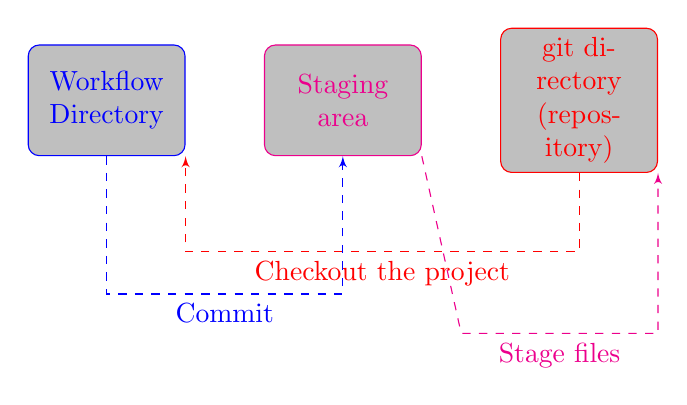
\begin{tikzpicture}[node distance = 2cm, auto]
		\node [blue, block] (st1) {Workflow Directory};
		\node [magenta, block, right of=st1, node distance=3cm] (st2) {Staging area};
		\node [red, block, right of=st2, node distance=3cm] (st3) {git directory (repository)};
%		\path [line] (st1) -- (st2);
%		\path [line] (st2) -- (st3);
		%% from st1 draw 1 unit down, then 2 units left (put a node), draw vertically up and then right to reach st1.west
		\path[red,line,dashed] (st3.south) -- ++(0,-1) -|  (st1.south east) node[pos=0.25,below]{Checkout the project};
		\path[blue,line,dashed] (st1.south) -- ++(0,-1.75) -|  (st2.south) node[pos=0.25,below]{Commit};
		\path[magenta,line,dashed] (st2.south east) -- ++(0.5,-2.25) -|  (st3.south east) node[pos=0.25,below]{Stage files};
		%% draw 1 unit down from st3.south then horizontally left and up to reach st2.south.
%		\path[line,dashed] (st3.south) -- +(0,-1) -|  (st2.south) node[pos=0.25,below]{Blah2};
	\end{tikzpicture}
		
\end{frame}





\begin{frame}[t]{Configurando o Git}
	
	\vspace{0.5em}
	
	\href{https://git-scm.com/book/pt-br/v2/Come\%C3\%A7ando-Configura\%C3\%A7\%C3\%A3o-Inicial-do-Git}{1.6 Começando - Configuração Inicial do Git <- clique aqui}
	
	\vspace{0.5em}
	Procure orientação de configuração com base no seu sistema operacional.
	
\end{frame}




\begin{frame}[t]{Mãos a obra}
	
	\vspace{0.5em}
	
	A solução git que vamos utilizar será o github.
	
	\vspace{1em}
	
	\href{https://github.com/new}{Criar novo repositório <- clique aqui}
	
\end{frame}


\begin{frame}[t]{Criando seu repositório}

	\centering
	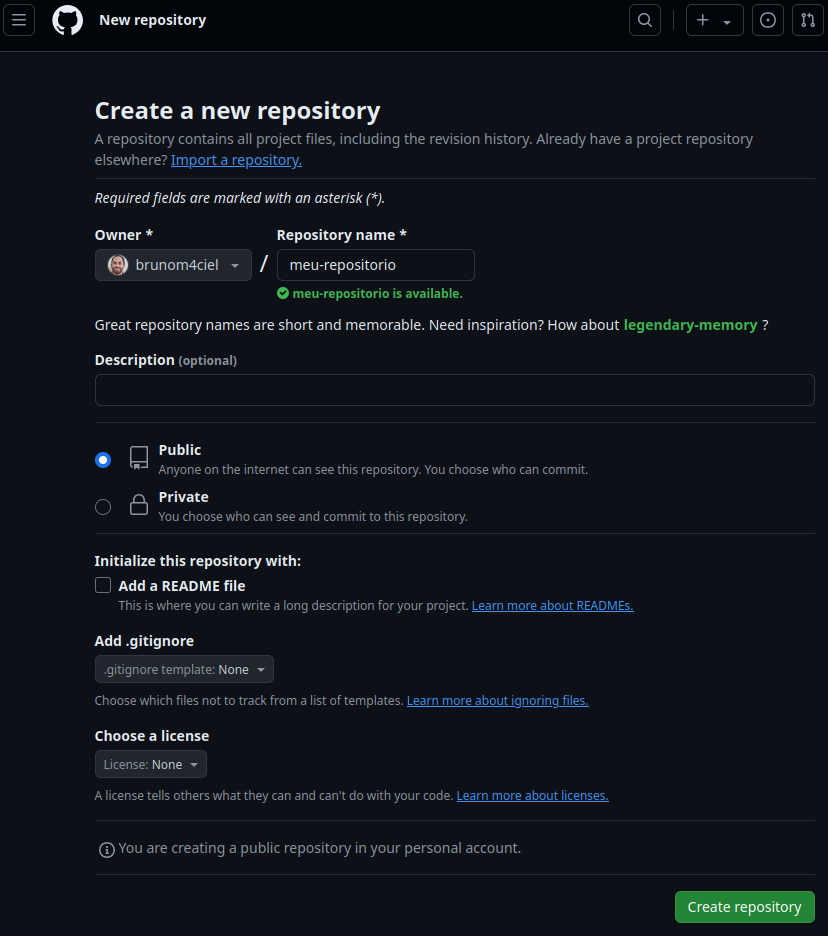
\includegraphics[scale=0.20]{imagens/fig-github-new.png}

\end{frame}



\begin{frame}[t]{Clonando um repositório existente}
	
	\vspace{1em}
	
	\fontsize{12pt}{15}\selectfont{
		\begin{itemize}%[<+->]
			\item Início
			\item Escolha um diretório para guardar o repositório. (procure um local que não tenha outros dados)
			\item Abra o terminal.
			\item Vá até o diretório escolhido.
			\item Execute o comando: \$ git clone git@github.com:brunom4ciel/material-python.git
			\item Executabdo com sucesso deve haver um diretório chamado material-python
			\item Fim
			
		\end{itemize}
	}\par
	\vspace{1em}
	
\end{frame}



\begin{frame}[t]{Fazendo mudanças}
	
	\vspace{1em}
	
	\fontsize{14pt}{19}\selectfont{
		\begin{itemize}%[<+->]  
			\item Cada arquivo pode estar em dois estados: tracked (monitorado) e untracked (não monitorado).
			
			\item Arquivos tracked são arquivos que estavam no último snapshot, eles podem estar em qualquer um dos três estados.
			
			\item Arquivos untracked são arquivos novos que ainda não estão sendo monitorados.
		\end{itemize}
	}\par
	\vspace{1em}
	
\end{frame}




\begin{frame}[t]{Adicionando arquivos e o primeiro commit}

	\fontsize{14pt}{19}\selectfont{
		\$ git add . -A\\
		\$ git commit -m 'versão inicial'\\
	}\par
	\vspace{1em}

	\fontsize{14pt}{19}\selectfont{
		\begin{itemize}%[<+->]  
			\item Com isso criamos um repositório local e mesmo sem a ajuda de um servidor externo podemos manter o histórico dos nossos arquivos. Ou seja, é possível usar o Git como LVCS.
		\end{itemize}
	}\par
	\vspace{1em}

\end{frame}





\begin{frame}[t]{Ciclo de vida de um arquivo}

	\vspace{1em}
	
	\centering
	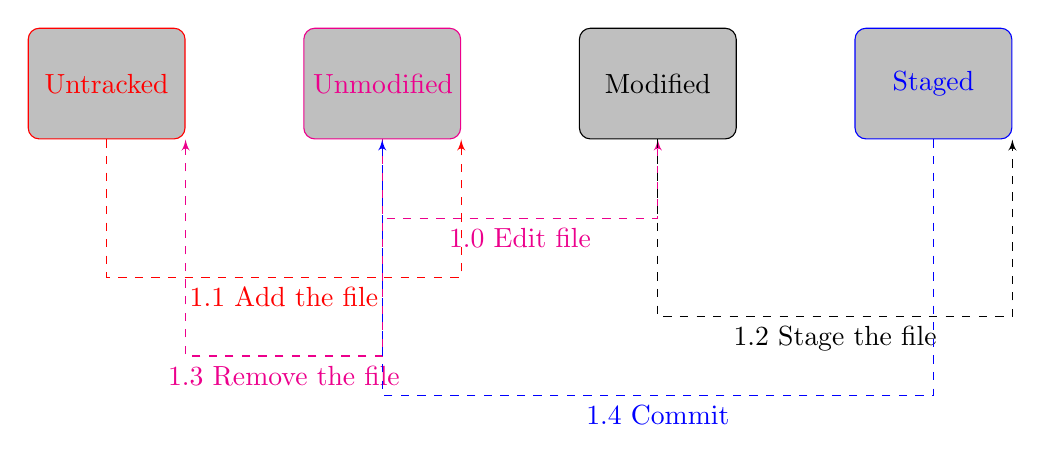
\begin{tikzpicture}[node distance = 2cm, auto]
		\node [red, block] (st1) {Untracked};
		\node [magenta, block, right of=st1, node distance=3.5cm] (st2) {Unmodified};
		\node [black, block, right of=st2, node distance=3.5cm] (st3) {Modified};
		\node [blue, block, right of=st3, node distance=3.5cm] (st4) {Staged};
		\path[magenta,line,dashed] (st2.south) -- ++(0,-1) -|  (st3.south) node[pos=0.25,below]{1.0 Edit file};
		\path[red,line,dashed] (st1.south) -- ++(0,-1.75) -| (st2.south east) node[pos=0.25,below]{1.1 Add the file};
		\path[black,line,dashed] (st3.south) -- ++(0,-2.25) -| (st4.south east) node[pos=0.25,below]{1.2 Stage the file};
		\path[magenta,line,dashed] (st2.south) -- ++(0,-2.75) -| (st1.south east) node[pos=0.25,below]{1.3 Remove the file};
		\path[blue,line,dashed] (st4.south) -- ++(0,-3.25) -|  (st2.south) node[pos=0.25,below]{1.4 Commit};
	\end{tikzpicture}

	
\end{frame}





\begin{frame}[t]{Checando o estado dos seus arquivos}
	
	\fontsize{14pt}{19}\selectfont{
		\$ git status\\
		\# On branch master\\
		nothing to commit (working directory clean)
	}\par
	\vspace{1em}
	
	\fontsize{14pt}{19}\selectfont{
		\begin{itemize}%[<+->]  
			\item se não houver modificações, o repositório está limpo.
		\end{itemize}
	}\par
	\vspace{1em}
	
\end{frame}






\begin{frame}[t]{Vamos fazer alguns testes}

	\fontsize{14pt}{19}\selectfont{
		\begin{itemize}%[<+->]  
			\item Adicione um arquivo ao repositório. Digite \$ git status e veja o resultado.
			
			\item \textit{\$ git add . -A} para incluir o arquivo modificado, use \textit{\$ git status}. Veja o resultado.
			
			\item Modifique o arquivo mais uma vez e \textit{\$ git status}. O que aconteceu?
			
		\end{itemize}
	}\par
	\vspace{1em}
	
\end{frame}





\begin{frame}[t]{O que aconteceu?}
	
	\fontsize{14pt}{19}\selectfont{
		\begin{itemize}%[<+->]  
			\item O Git faz um snapshot do arquivo na hora que você dá um \textit{\$ git add}.
			
			\item Se você commitar agora, você irá commitar a versão antiga do arquivo, do jeito que ele estava no último \textit{\$ git add} feito.
			
			\item É necessário outro \textit{\$ git add} para que as alterações sejam feitas.
			
		\end{itemize}
	}\par
	\vspace{1em}
	
\end{frame}





\begin{frame}[t]{Vendo o histórico de commits}
	
	\fontsize{14pt}{19}\selectfont{
		\$ git log\\

	}\par
	\vspace{1em}

\fontsize{10pt}{15}\selectfont{
commit a7df3cbe37cc9762c9bc4fa16853d459889c8706 (HEAD -> main, origin/main, origin/HEAD)\\
Author: Avneesh Agarwal <avneeshagarwal0612@gmail.com>\\
Date:   Wed Nov 10 12:05:12 2021 +0530\\
\vspace{1em}
Delete README.md\\
\vspace{1em}
commit 10d0879b76f21460a36bf8d246f95f853c08c78a\\
Author: Your Name <avneeshagarwal0612@gmail.com>\\
Date:   Thu Sep 23 11:59:25 2021 +0530\\
\vspace{1em}
upgrade packages\\

	}\par
\vspace{1em}


\end{frame}





\begin{frame}[t]{Modificando seu último commit}
	
	\fontsize{14pt}{19}\selectfont{
		\begin{itemize}%[<+->]  
			\item Alterando só a mensagem do commit:\\
			
			\textit{\$ git commit --amend}
			
			\item Adicionando um arquivo ao último commit:\\
			
			\textit{\$ git commit -m 'initial commit'}\\
			\textit{\$ git add README.md}\\
			\textit{\$ git commit --amend}
		\end{itemize}
	}\par
	\vspace{1em}
	
\end{frame}



\begin{frame}[t]{Removendo um arquivo staged}
	
	\fontsize{14pt}{19}\selectfont{
		\begin{itemize}%[<+->]  
			\item \textit{\$ git reset HEAD README.md}

		\end{itemize}
	}\par
	\vspace{1em}
	
\end{frame}




\begin{frame}[t]{Repositórios remoto}
	
	\fontsize{14pt}{19}\selectfont{
		\begin{itemize}%[<+->]  
			\item \textit{\$ git remote -v} mostra as URLs do repositório.
			
		\end{itemize}
	}\par
	\vspace{1em}
	
\end{frame}




\begin{frame}[t]{Puxando informações do novo repositório}
	
	\fontsize{14pt}{19}\selectfont{
		\begin{itemize}%[<+->]  
			\item Um \textit{\$ git pull} faz um fetch e depois um merge, incluindo as modificações feitas no repositório pb no seu repositório local.
			
		\end{itemize}
	}\par
	\vspace{1em}
	
\end{frame}





\begin{frame}[t]{Enviando suas modificações ao repositório}
	
	\fontsize{14pt}{19}\selectfont{
		\begin{itemize}%[<+->]
			\item \textit{\$ git push origin main}
			
		\end{itemize}
	}\par
	\vspace{1em}
	
	*obs: Você precisa de acesso a escrita para poder enviar informações num repositório remoto.
\end{frame}






\begin{frame}[t]{O que são branchs?}
	
	\fontsize{14pt}{19}\selectfont{
		\begin{itemize}%[<+->]
			\item \textit{\$ git branch testing}
			
		\end{itemize}
	}\par
	\vspace{1em}
	
	*obs: Agora criamos um novo branch, que aponta para a última modificação feita.
	
\end{frame}





\begin{frame}[t]{Como o Git sabe qual é o branch atual?}
	
	\fontsize{14pt}{19}\selectfont{
		\begin{itemize}%[<+->]
			\item O ponteiro \textbf{HEAD} indica qual o branch que está sendo usado.
			
			\item Para mudar o HEAD de lugar, usamos: \textit{\$ git checkout testing}
			
		\end{itemize}
	}\par
	\vspace{1em}
	
\end{frame}





\begin{frame}[t]{Merge}
	
	\fontsize{14pt}{19}\selectfont{
		\begin{itemize}%[<+->]
			\item Vamos fazer um merge nas modificações do testing na branch main.
			
			\textit{\$ git checkout main}\\
			\textit{\$ git merge testing}
			
			
		\end{itemize}
	}\par
	\vspace{1em}
	
\end{frame}




\begin{frame}[t]{Rebase}
	
	\fontsize{14pt}{19}\selectfont{
		\begin{itemize}%[<+->]
			\item Outra maneira de juntar seu trabalho a um outro branch.
			
			\textit{\$ git checkout experiment}\\
			\textit{\$ git rebase main}
			
			
		\end{itemize}
	}\par
	\vspace{1em}
	
\end{frame}





\begin{frame}[t]{Delete branch}
	
	\fontsize{14pt}{19}\selectfont{
		\begin{itemize}%[<+->]
			\item Para excluir uma branch.
			
			\textit{\$ git branch -D testing}\\
			
		\end{itemize}
	}\par
	\vspace{1em}
	
\end{frame}




\begin{frame}[t]{Clonar branch}
	
	\fontsize{14pt}{19}\selectfont{
		\begin{itemize}%[<+->]
			\item Para excluir uma branch.
			
			\textit{\$ git checkout -b testingfix origin/testingfix}\\
			
		\end{itemize}
	}\par
	\vspace{1em}
	
\end{frame}


